% ============================================================================
%  Thesis Defense Presentation — UTEC / GINIA (Final Production Version)
%  Efficient Multi-Temporal Building Change Detection
%  with Reduced-Rank Linear Attention
% ============================================================================
\documentclass[aspectratio=169]{beamer}

% ---------- Theme ----------
\usetheme{Madrid}
\usecolortheme{default}

% ---------- UTEC Identity Colors ----------
\definecolor{utecblue}{HTML}{003262}
\definecolor{pastelorange}{rgb}{1.00,0.85,0.65}
\definecolor{charcoal}{HTML}{222222}

\setbeamercolor{structure}{fg=utecblue}
\setbeamercolor{palette primary}{bg=utecblue,fg=white}
\setbeamercolor{palette secondary}{bg=utecblue!80,fg=white}
\setbeamercolor{palette tertiary}{bg=utecblue!60,fg=white}
\setbeamercolor{palette quaternary}{bg=utecblue,fg=white}
\setbeamercolor{frametitle}{bg=utecblue,fg=white}
\setbeamercolor{title}{bg=utecblue,fg=white}

% ---------- Packages ----------
\usepackage[utf8]{inputenc}
\usepackage{graphicx}
\usepackage{amsmath,amssymb}
\usepackage[table]{xcolor}
\usepackage{colortbl}
\usepackage{multirow}
\usepackage{booktabs}
\usepackage{tikz}
\usepackage{times}
\usepackage{helvet}
\usepackage{courier}
\usefonttheme{serif}

\graphicspath{{images/}{plots/}}

\setlength{\abovedisplayskip}{3pt}
\setlength{\belowdisplayskip}{3pt}
\setlength{\abovedisplayshortskip}{1pt}
\setlength{\belowdisplayshortskip}{1pt}

\setbeamertemplate{navigation symbols}{}
\setbeamerfont{normal text}{size=\small}
\setbeamertemplate{itemize items}[circle]

% ---------- Title Info ----------
\title[Efficient BCD via Reduced-Rank Linear Attention]{%
  Enhancing Computational Efficiency in\\
  Multi-Temporal Building Change Detection\\
  via Reduced-Rank Linear Attention}

\author[R. Acuña Villogas]{Ricardo Amiel Acuña Villogas}

\institute[UTEC -- GINIA]{%
  \textbf{Universidad de Ingeniería y Tecnología (UTEC)}\\
  Data Science Bachelor's Thesis Defense\\[4pt]
  \small
  \textit{Thesis Advisor:}\; PhD.\ Rensso Víctor Hugo Mora Colque\\[2pt]
  \textit{Co-Advisors:}\;
    PhD.\ Cristian José López del Álamo\;\textbar\;
    PhD.\ Germain García Zanabria
}

\date{June 30, 2026}

% ============================================================
\begin{document}
% ============================================================

% ----------------------------------------------------------
% FRAME 1 — Title
% ----------------------------------------------------------
\begin{frame}
  \titlepage
\end{frame}

% ----------------------------------------------------------
% FRAME 2 — Outline
% ----------------------------------------------------------
\begin{frame}{Defense Roadmap}
\tableofcontents
\end{frame}

% ==========================================================
\section{Motivation}
% ==========================================================

\begin{frame}{Building Change Detection}

\begin{columns}[T]
% ---------- Left column ----------
\begin{column}{0.42\textwidth}

\includegraphics[
  width=\linewidth,
  height=0.7\textheight,
  keepaspectratio
]{vectorized-LEVIRCD.pdf}

\end{column}

% ---------- Right column ----------
\begin{column}{0.48\textwidth}

\small
\textbf{Building Change Detection (BCD)} compares \textbf{bi-temporal satellite images} to identify construction, demolition, or structural change.

\vspace{0.4cm}

\textbf{Why it matters}
\begin{itemize}
    \item Urban growth monitoring.
    \item Disaster response.
    \item Security and regulation.
    \item Planning and poverty analysis.
\end{itemize}

\end{column}
\end{columns}

\vspace{0.3cm}
\footnotesize
\tiny{\textit{A Spatial-Temporal Attention-Based Method and a New Dataset for Remote Sensing Image Change Detection. (Zheng et al.)}}

\end{frame}

% ----------------------------------------------------------
% FRAME 3 — Motivation: VHR Context
% ----------------------------------------------------------
\begin{frame}{Motivation: VHR Urban Monitoring in the Global South}

\begin{columns}[T]
\begin{column}{0.48\textwidth}
\centering
\includegraphics[height=0.55\textheight,keepaspectratio]{PeruSat.png}\\
\vspace{2pt}
{\tiny\color{charcoal}\textit{Conida PeruSat-1 sample)}}
\end{column}

\begin{column}{0.48\textwidth}
\centering
\includegraphics[height=0.55\textheight,keepaspectratio]{LandCover.png}\\
\vspace{2pt}
{\tiny{Land cover changes in Lima Metropolitan Area for the years 2008 and 2021}}
\end{column}
\end{columns}

\end{frame}

% ==========================================================
\section{Problem Statement}
% ==========================================================

% ----------------------------------------------------------
% FRAME 4 — Problem: The Quadratic Bottleneck (Layout & Text Flow Fixed)
% ----------------------------------------------------------
\begin{frame}{Problem Statement: The Quadratic Attention Bottleneck}

\begin{columns}[T]
\begin{column}{0.52\textwidth}
\centering
\includegraphics[height=0.58\textheight,keepaspectratio]{Attention.png}\\
\vspace{4pt}
{\tiny\color{charcoal}\textit{Fan et al., Breaking the Low-Rank Dilemma via Linear Attention, ICLR 2025}}
\end{column}
\hfill
\begin{column}{0.44\textwidth}
\vspace{0.1cm}
\textbf{\color{utecblue}Computational Constraints:}
\vskip 0.1cm
\small
\begin{itemize}
    \item High computational cost: $\mathcal{O}(N^2)$.
    \item Large memory footprint.
    \item Small feasible batch sizes.
    \item Bi-temporal processing doubles computation.
    \item Limits deployment on large or OOD datasets.
\end{itemize}

\end{column}
\end{columns}

\end{frame}

\begin{frame}{Main Goal}

\begin{center}
{\Large\bfseries
Design a computationally efficient attention mechanism that reduces cost while preserving segmentation accuracy.
}
\end{center}

\end{frame}

\begin{frame}{Goals}
\begin{itemize}
    \item Reduce VRAM usage and FLOPs in the encoder.
    \item Increase feasible batch sizes for large-scale BCD training.
    \item Maintain comparable performance on six different BCD datasets.
    \item \textbf{Scope}:  Train and validation on public benchmarks LEVIR-CD/LEVIR-CD+ (Zheng et al.) and DSIFN-CD (Zhang et al.),  WHU-CD (Ji et al.), SYSU-CD(Shi et al.) and S2Looking (Shen et al.).
\end{itemize}
\end{frame}

% ----------------------------------------------------------
% FRAME — Contributions
% ----------------------------------------------------------
\begin{frame}{Contributions}
\begin{itemize}
    \item \textbf{A lightweight change detection model.} We propose RALA-ChangeFormer, a hierarchical Siamese Transformer that replaces the quadratic multi-head self-attention of ChangeFormer with rank-augmented linear attention, reducing attention-related peak GPU memory consumption and enabling larger, more stable training configurations without sacrificing segmentation accuracy.
    \item \textbf{A complete and robust benchmarking.} We conduct a systematic cross-domain evaluation across six geographically and methodologically diverse datasets (LEVIR-CD, DSIFN-CD, WHU-CD, LEVIR-CD+, SYSU-CD, and S2Looking), jointly reporting accuracy and efficiency metrics (FLOPs, peak memory, maximum feasible batch size, and training throughput) to characterize the generalization boundaries of rank-augmented linear attention.
    \item \textbf{A peer-reviewed publication.} The core of this work has been accepted and published at the 21st International Conference on Computer Vision Theory and Applications (VISAPP 2026), validating the relevance and soundness of the proposed approach.
    \item \textbf{An ongoing journal extension.} Building on the accepted conference paper, we are currently developing an extended version for a journal submission, broadening the experimental evaluation and deepening the analysis of the efficiency--accuracy trade-offs reported throughout this thesis.
\end{itemize}
\end{frame}

% ==========================================================
\section{Related Work \& Baseline}
% ==========================================================

% ----------------------------------------------------------
% FRAME 5 — State of the Art
% ----------------------------------------------------------
\begin{frame}{State of the Art in Building Change Detection (BCD)}

\begin{center}
\begin{minipage}{\linewidth}
\centering
\begin{tikzpicture}
  \node[anchor=south west, inner sep=0] (img) at (0,0)
    {\includegraphics[width=\linewidth,height=0.60\textheight,keepaspectratio]{SOTA.png}};
  \draw[dashed,line width=1.2pt,rounded corners=4pt,utecblue]
    (0.1,0.40) rectangle (14.3,1.55);
\end{tikzpicture}
\vspace{2pt}
{\tiny\color{charcoal}\textit{Bandara \& Patel, ChangeFormer, IGARSS 2022}}
\end{minipage}
\end{center}

\end{frame}

% ----------------------------------------------------------
% FRAME 6 — Baseline: ChangeFormer Architecture (Vertical Center and Enlarged Figure)
% ----------------------------------------------------------
\begin{frame}{Baseline: ChangeFormer Architecture}

\begin{columns}[c] % Alineación vertical perfectamente centrada
\begin{column}{\textwidth}
\centering
\includegraphics[width=\linewidth,height=0.74\textheight,keepaspectratio]{ChangeFormer.png}\\
\vspace{2pt}
\tiny{\textit{A Transformer-based Siamese Network for Change Detection} (Bandara et al.)}
\end{column}
\end{columns}

\end{frame}

% ==========================================================
\section{Proposed Method}
% ==========================================================

% ----------------------------------------------------------
% FRAME 7 — RALA-CF Architecture (Vertical Center and Enlarged Figure)
% ----------------------------------------------------------
\begin{frame}{Proposed Architecture: RALA-CF Drop-in Substitution}

\begin{columns}[c] % Alineación vertical perfectamente centrada
\begin{column}{0.58\textwidth}
\centering
\includegraphics[width=\linewidth,height=0.74\textheight,keepaspectratio]{ChangeFormer.png}\\
\vspace{2pt}
{\tiny\color{charcoal}\textit{A Transformer-based Siamese Network for Change Detection.}}
\end{column}

\begin{column}{0.38\textwidth}
{\footnotesize\raggedright
\textbf{\color{utecblue}Drop-In Engineering Scope:}
\vskip 0.1cm
\begin{itemize}
  \item MHSA systematically replaced at \textbf{all 4} Siamese levels.
  \item Feed-Forward Networks (FFN): \textbf{Unchanged}.
  \item Inductive Skip Connections: \textbf{Preserved}.
  \item Final Segmentation Decoder: \textbf{Intact}.
\end{itemize}

\vskip 0.5cm
\textbf{\color{charcoal}Complexity Profile Per Level:}\\
\hspace{0.5em}Standard MHSA:\; $\mathcal{O}(N_l^2\,d)$\\
\hspace{0.5em}Rank-Augmented RALA:\; $\mathcal{O}(N_l\,d^2)$\\[4pt]
Given that $N_l \gg d$ holds at every hierarchical layer, it delivers a sustained \textbf{sub-quadratic memory and operational profile}.
}
\end{column}
\end{columns}

\end{frame}

% ----------------------------------------------------------
% FRAME 8 — Mathematical Innovation: RALA Core
% ----------------------------------------------------------
\begin{frame}{Mathematical Innovation: Rank-Augmented Linear Attention}

\begin{columns}[T]
\begin{column}{0.42\textwidth}
\centering
\includegraphics[width=\linewidth,height=0.58\textheight,keepaspectratio]{RALA.png}\\
\vspace{2pt}
{\tiny\color{charcoal}\textit{Fan et al., ICLR 2025}}
\end{column}

\begin{column}{0.55\textwidth}
\footnotesize
\textbf{\color{utecblue}Global Query Descriptor (Context Ponderation):}
\[
Q_g = \tfrac{1}{N}\textstyle\sum_{i=1}^{N} Q_i
\]

\textbf{\color{utecblue}Differential Token Re-weighting Coefficients:}
\[
\alpha_j = N\cdot\frac{\exp\!\bigl(Q_g\,\kappa(K_j)^\top\bigr)}{\sum_{m}\exp\!\bigl(Q_g\,\kappa(K_m)^\top\bigr)}, \quad \textstyle\sum_j\alpha_j=N
\]

\textbf{\color{utecblue}Rank-Augmented Key-Value Mixing Buffer:}
\[
B = \textstyle\sum_{j=1}^{N} \alpha_j\,\kappa(K_j)^\top V_j \quad \in \mathbb{R}^{d \times d}
\]

\textbf{\color{utecblue}Hadamard Output Feature Modulation:}
\[
Y_i = \phi(X_i)\odot\bigl(\kappa(Q_i)\,B\bigr)
\]
\end{column}
\end{columns}

\vskip 0.2cm
\hrule
\vskip 0.15cm
\footnotesize
\textbf{\color{utecblue}Architectural Invariant}: The pixel-dependent transformation layer $\phi(\cdot)$ effectively breaks the low-rank capacity ceiling ($\operatorname{Rank}(Y)\not\le d$). This architectural step fully restores multi-temporal semantic expressiveness while remaining within linear time boundaries $\mathcal{O}(Nd^2)$.

\end{frame}

\begin{frame}{Datasets: LEVIR-CD}

\begin{center}
\includegraphics[
  width=0.95\linewidth,
  height=0.7\textheight,
  keepaspectratio
]{LEVIR2.png}
\end{center}

\vspace{0.3cm}

\vspace{0.2cm}
\footnotesize
\tiny{\textit{A Spatial-Temporal Attention-Based Method and a New Dataset for Remote Sensing Image Change Detection} (Zhang et al.)}

\end{frame}


\begin{frame}{Datasets: DSIFN-CD}

\begin{center}
\includegraphics[
  width=0.95\linewidth,
  height=0.7\textheight,
  keepaspectratio
]{DSIFN2.png}
\end{center}

\vspace{0.3cm}

\vspace{0.2cm}
\footnotesize
\tiny{\textit{A Dense Siamese Network for Change Detection in Remote Sensing Images} (Zhang et al.)}

\end{frame}

% ==========================================================
\section{Experiments \& Results}
% ==========================================================

% ----------------------------------------------------------
% FRAME 9a — Quantitative: Part I (Cell Color Superposition Hot-Fixed)
% ----------------------------------------------------------
\begin{frame}{Quantitative Evaluation: Primary Benchmarks (Part I)}

\centering

\renewcommand{\arraystretch}{1.15}
\small
\begin{tabular}{|l|l|c|c|c|c|}
\hline
\textbf{Target Benchmark} & \textbf{Architecture Baseline} & \textbf{Precision} & \textbf{$F_1$-Score} & \textbf{IoU} & \textbf{OA (\%)} \\
\hline
\hline
\multirow{5}{*}{\textbf{LEVIR-CD}} & FC-EF & 86.91 & 83.40 & 71.53 & 98.39 \\ \cline{2-6}
                          & SNUNet-CD & 89.18 & 88.16 & 78.83 & 98.87 \\ \cline{2-6}
                          & BIT & 89.24 & 89.31 & 80.68 & 98.92 \\ \cline{2-6}
                          & ChangeFormer & \textbf{92.05} & \textbf{90.40} & \textbf{82.48} & \textbf{99.04} \\ \cline{2-6}
                          & \textbf{Ours (RALA-CF)} & \cellcolor{pastelorange} 90.08 & \cellcolor{pastelorange} 89.67 & \cellcolor{pastelorange} 81.60 & \cellcolor{pastelorange} 98.99 \\
\hline
\hline
\multirow{5}{*}{\textbf{DSIFN-CD}} & FC-EF & 72.61 & 61.09 & 43.98 & 88.59 \\ \cline{2-6}
                          & SNUNet-CD & 60.60 & 66.18 & 49.45 & 87.34 \\ \cline{2-6}
                          & BIT & 68.36 & 69.26 & 52.97 & 89.41 \\ \cline{2-6}
                          & ChangeFormer & \textbf{88.48} & \textbf{86.67} & \textbf{76.48} & \textbf{95.56} \\ \cline{2-6}
                          & \textbf{Ours (RALA-CF)} & \cellcolor{pastelorange} 84.97 & \cellcolor{pastelorange} 84.07 & \cellcolor{pastelorange} 73.96 & \cellcolor{pastelorange} 92.44 \\
\hline
\end{tabular}

\end{frame}

% ----------------------------------------------------------
% FRAME 9b — Quantitative: Part II (Cell Color Superposition Hot-Fixed)
% ----------------------------------------------------------
\begin{frame}{Quantitative Evaluation: Cross-Domain Benchmarks (Part II)}

\centering

\renewcommand{\arraystretch}{1.15}
\small
\begin{tabular}{|l|l|c|c|c|c|}
\hline
\textbf{Target Benchmark} & \textbf{Architecture Baseline} & \textbf{Precision} & \textbf{$F_1$-Score} & \textbf{IoU} & \textbf{OA (\%)} \\
\hline
\hline
\multirow{2}{*}{\textbf{WHU-CD}}    & ChangeFormer & 84.87 & 87.45 & 77.70 & \textbf{99.11} \\ \cline{2-6}
                           & \textbf{Ours (RALA-CF)} & \cellcolor{pastelorange}\textbf{90.14} & \cellcolor{pastelorange}\textbf{87.85} & \cellcolor{pastelorange}\textbf{78.33} & \cellcolor{pastelorange} 99.06 \\
\hline
\hline
\multirow{2}{*}{\textbf{LEVIR-CD+}} & ChangeFormer & 79.97 & \textbf{80.65} & \textbf{67.58} & \textbf{98.44} \\ \cline{2-6}
                           & \textbf{Ours (RALA-CF)} & \cellcolor{pastelorange}\textbf{80.20} & \cellcolor{pastelorange} 80.24 & \cellcolor{pastelorange} 67.01 & \cellcolor{pastelorange} 98.39 \\
\hline
\hline
\multirow{2}{*}{\textbf{SYSU-CD}}   & ChangeFormer & 77.90 & 78.81 & \textbf{65.03} & \textbf{90.12} \\ \cline{2-6}
                           & \textbf{Ours (RALA-CF)} & \cellcolor{pastelorange}\textbf{82.10} & \cellcolor{pastelorange}\textbf{78.02} & \cellcolor{pastelorange} 63.97 & \cellcolor{pastelorange}\textbf{90.12} \\
\hline
\hline
\multirow{2}{*}{\textbf{S2Looking}} & ChangeFormer & \textbf{72.14} & \textbf{61.89} & \textbf{45.77} & 84.55 \\ \cline{2-6}
                           & \textbf{Ours (RALA-CF)} & \cellcolor{pastelorange} 70.02 & \cellcolor{pastelorange} 60.39 & \cellcolor{pastelorange} 43.25 & \cellcolor{pastelorange}\textbf{99.16} \\
\hline
\end{tabular}

\end{frame}

% ----------------------------------------------------------
% FRAME 10 — Computational Efficiency
% ----------------------------------------------------------
\begin{frame}{Computational Efficiency}

\centering
\textbf{\color{utecblue}Resource Profile ($256{\times}256$, Batch 16)}
\vskip 0.3cm

\renewcommand{\arraystretch}{1.25}
\footnotesize
\begin{tabular}{|l|c|c|c|}
\hline
\textbf{Method} & \textbf{Params (M)} & \textbf{GFLOPs} & \textbf{VRAM (GB)} \\
\hline\hline
FC-EF        &  1.35 &   3.48 &  1.84 \\ \hline
SNUNet-CD    & 12.04 &  14.86 &  5.67 \\ \hline
BIT          & 11.05 &  17.22 &  5.13 \\ \hline
ChangeFormer & 247   & 248.77 & 27 \\ \hline
\rowcolor{pastelorange}
\textbf{Ours (RALA-CF)} & \textbf{243} & \textbf{228.62} & \textbf{21} \\ \hline
\end{tabular}

\vskip 0.5cm
\footnotesize
\begin{itemize}
  \item $-$22.2\% peak VRAM \quad $-$8.1\% GFLOPs.
  \item Equivalent capacity; gains from attention restructuring.
\end{itemize}

\end{frame}

% ----------------------------------------------------------
% FRAME 10b — OOM-Boundary Scaling
% ----------------------------------------------------------
\begin{frame}{OOM-Boundary Scaling}

\centering
\textbf{\color{utecblue}Max Feasible Batch Size Before OOM}
\vskip 0.3cm

\renewcommand{\arraystretch}{1.25}
\footnotesize
\begin{tabular}{|l|c|c|c|}
\hline
\textbf{Resolution} & \textbf{ChangeFormer} & \textbf{Ours (RALA-CF)} & \textbf{Gain} \\
\hline\hline
$256{\times}256$    & 32 & \textbf{48} & $+50\%$ \\ \hline
$512{\times}512$    &  8 & \textbf{12} & $+50\%$ \\ \hline
$1024{\times}1024$  &  2 & \textbf{3}  & $+50\%$ \\ \hline
\end{tabular}

\vskip 0.5cm
\footnotesize
\begin{itemize}
  \item Attention maps $\approx 1/3$ of peak VRAM.
  \item Removing $N_l{\times}N_l$ storage $\Rightarrow$ uniform $+50\%$ batch headroom.
  \item Unlocks native $1024{\times}1024$ training.
\end{itemize}

\end{frame}

% ----------------------------------------------------------
% FRAME 11 — Qualitative: WHU-CD (Expanded Column to prevent leaking)
% ----------------------------------------------------------
\begin{frame}{Qualitative Analysis: WHU-CD (Nadir Aerial Geometry)}

\begin{columns}[T]
\begin{column}{0.68\textwidth}
\centering

\includegraphics[width=\linewidth,height=0.68\textheight,keepaspectratio]{plots/qualitative_WHU_CD.pdf}
\end{column}
\begin{column}{0.29\textwidth}
\vspace{0.1cm}
\footnotesize\raggedright
\textbf{\color{utecblue}Error Metric Maps:}
\vskip 0.05cm
{\color{white}\rule{6pt}{6pt}} TP (White)\quad {\color{black}\rule{6pt}{6pt}} TN (Black)\\
{\color{red}\rule{6pt}{6pt}} FP (Red)\quad {\color{blue}\rule{6pt}{6pt}} FN (Blue)

\vskip 0.3cm
\textbf{\color{utecblue}Nadir Geometry Insights:}
\vskip 0.1cm
\begin{itemize}
  \item Cenital scans eliminate perspective structural shifts.
  \item High $0.3$\,m/px resolution handles complex boundaries.
  \item Rank-augmented $\alpha_j$ preserves fine building masks.
\end{itemize}
\end{column}
\end{columns}

\vskip 0.05cm
\centering
{\tiny Rows denote random independent scene configurations. Columns group: Pre-image $\mid$ Post-image $\mid$ Target Label $\mid$ ChangeFormer $\mid$ Ours (RALA-CF)}

\end{frame}

% ----------------------------------------------------------
% FRAME 12 — Qualitative: S2Looking Part I (Split into 2 slides)
% ----------------------------------------------------------
\begin{frame}{Qualitative Analysis: S2Looking (Oblique Geometry Failure)}

\begin{columns}[T]
\begin{column}{0.68\textwidth}
\centering

\includegraphics[width=\linewidth,height=0.68\textheight,keepaspectratio]{plots/qualitative_S2Looking.pdf}
\end{column}
\begin{column}{0.29\textwidth}
\vspace{0.1cm}
\footnotesize\raggedright
\textbf{\color{utecblue}Geometric Failure Analysis:}
\vskip 0.15cm
\begin{itemize}
  \item Oblique angles trigger structural parallax displacement.
  \item Unchanged tall facades display artificial offsets.
  \item Ring-shaped false-positive halos degrade accuracy.
\end{itemize}
\end{column}
\end{columns}

\vskip 0.05cm
\centering
{\tiny Rows denote random independent scene configurations. Columns group: Pre-image $\mid$ Post-image $\mid$ Target Label $\mid$ ChangeFormer $\mid$ Ours (RALA-CF)}

\end{frame}

% ----------------------------------------------------------
% FRAME 12.5 — Oblique-Angle Parallax Mechanism (Image A vs Image B)
% ----------------------------------------------------------
\begin{frame}{Oblique Geometry: Why Parallax Triggers False Change}

\begin{columns}[c]
\begin{column}{0.52\textwidth}
\centering
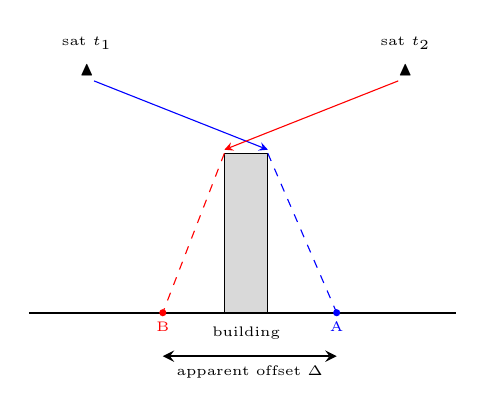
\begin{tikzpicture}[scale=0.92, >=stealth, font=\scriptsize]
  \draw[thick] (-0.3,0) -- (5.6,0);
  \fill[gray!30,draw=black] (2.4,0) rectangle (3.0,2.2);
  \node[font=\tiny] at (2.7,-0.28) {building};
  \node at (0.5,3.35) {$\blacktriangle$};
  \node at (4.9,3.35) {$\blacktriangle$};
  \node[font=\tiny] at (0.5,3.72) {sat $t_1$};
  \node[font=\tiny] at (4.9,3.72) {sat $t_2$};
  \draw[blue,->] (0.6,3.2) -- (3.0,2.25);
  \draw[red,->]  (4.8,3.2) -- (2.4,2.25);
  \draw[blue,dashed] (3.0,2.2) -- (3.95,0);
  \draw[red,dashed]  (2.4,2.2) -- (1.55,0);
  \fill[blue] (3.95,0) circle (1.4pt); \node[blue,font=\tiny,below] at (3.95,0) {A};
  \fill[red]  (1.55,0) circle (1.4pt); \node[red,font=\tiny,below] at (1.55,0) {B};
  \draw[<->,thick] (1.55,-0.6) -- (3.95,-0.6);
  \node[font=\tiny,below] at (2.75,-0.6) {apparent offset $\Delta$};
\end{tikzpicture}
\end{column}
\begin{column}{0.46\textwidth}
\footnotesize
\textbf{\color{utecblue}Image A ($t_1$) vs. Image B ($t_2$):}
\vskip 0.2cm
\begin{itemize}
  \item Acquired at different off-nadir angles.
  \item Tall structures project to shifted ground positions (A $\neq$ B).
  \item Offset $\Delta$ on an \textbf{unchanged} building $\Rightarrow$ ring-shaped false-positive halo.
\end{itemize}
\end{column}
\end{columns}

\end{frame}

% ----------------------------------------------------------
% FRAME 14 — S2Looking Architectural Limits (keywords + qualitative highlight)
% ----------------------------------------------------------
\begin{frame}{S2Looking: Architectural Limits}

\begin{columns}[c]
\begin{column}{0.48\textwidth}
\footnotesize
\textbf{\color{red!80!black}The Parallax Limit:}
\vskip 0.25cm
\begin{itemize}
  \item \textbf{Error-pattern invariance}: ChangeFormer $\equiv$ RALA-CF halos.
  \item \textbf{Backbone-level cause}: SegFormer-B2, not attention.
  \item \textbf{Irreducible by attention}: requires geometric / depth alignment.
\end{itemize}
\end{column}
\begin{column}{0.50\textwidth}
\centering

\includegraphics[width=\linewidth,height=0.62\textheight,keepaspectratio]{plots/qualitative_S2Looking.pdf}\\
{\tiny\color{charcoal}Identical FP halos (red) in the ChangeFormer and RALA-CF columns.}
\end{column}
\end{columns}

\end{frame}

% ==========================================================
\section{Conclusions}
% ==========================================================

% ----------------------------------------------------------
% FRAME 13 — Conclusions
% ----------------------------------------------------------
\begin{frame}{Core Empirical Milestones}

\footnotesize
\begin{itemize}
  \item Quadratic $\to$ linear encoder attention: $\mathcal{O}(N_l^2 d) \to \mathcal{O}(N_l d^2)$.
  \item Rank-augmentation $+$ Hadamard $\phi(\cdot)$ prevent low-rank collapse.
  \item Near-parity across 6 datasets: mean $-0.94$\,pp F1; surpasses ChangeFormer on WHU-CD.
  \item Efficiency: $-22.2\%$ VRAM, $-8.1\%$ GFLOPs, uniform $+50\%$ batch size.
\end{itemize}

\vskip 0.6cm
\centering
\footnotesize\color{charcoal}
Rank-augmented linear attention: a mathematically sound, non-heuristic path to efficient multi-temporal remote sensing.

\end{frame}

% ----------------------------------------------------------
% FRAME 16 — Identified Research Limitations
% ----------------------------------------------------------
\begin{frame}{Identified Research Limitations}

\begin{columns}[c]
\begin{column}{0.50\textwidth}
\footnotesize
\begin{itemize}
  \item \textbf{Geometric parallax} (S2Looking): a backbone limit, not solvable by attention alone.
  \item \textbf{Multi-class label mismatch} (SYSU-CD): false positives on non-building change.
  \item \textbf{Hardware floor}: full-resolution training on $\leq 8$\,GB GPUs still out of reach.
\end{itemize}
\end{column}
\begin{column}{0.48\textwidth}
\centering

\includegraphics[width=\linewidth,height=0.62\textheight,keepaspectratio]{plots/qualitative_SYSU_CD.pdf}\\
{\tiny\color{charcoal}SYSU-CD: false positives (red) on non-building multi-class change.}
\end{column}
\end{columns}

\end{frame}

% ==========================================================
\section{Future Work}
% ==========================================================

% ----------------------------------------------------------
% FRAME 14 — Future Research
% ----------------------------------------------------------
\begin{frame}{Technical Foundations and Extensions}

\footnotesize
\begin{enumerate}
  \item \textbf{Dynamic rank adaptation}: online SVD tracking of the KV buffer $B$.
  \item \textbf{Geometric pre-alignment}: stereophotogrammetric / DEM depth to correct parallax before tokenization.
  \item \textbf{Multi-temporal ingestion}: extend $Q_g$ to $T > 2$ acquisitions for continuous construction monitoring.
\end{enumerate}

\end{frame}

% ----------------------------------------------------------
% FRAME 18 — Regional Benchmarks and Local Deployment
% ----------------------------------------------------------
\begin{frame}{Regional Benchmarks and Local Deployment}

\begin{columns}[c]
\begin{column}{0.52\textwidth}
\footnotesize
\begin{enumerate}
  \item \textbf{Latin American BCD benchmark}: PeruSAT-1 datasets over Lima or other states, expand to Sao Paulo, Bogotá.
  \item \textbf{Informal-settlement ontologies}: metrics calibrated for self-construction monitoring.
  \item \textbf{Operational tooling}: city-scale mosaicking for planning and risk assessment.
\end{enumerate}
\end{column}
\begin{column}{0.46\textwidth}
\centering
\includegraphics[width=\linewidth,height=0.62\textheight,keepaspectratio]{PeruSat.png}\\
{\tiny\color{charcoal}Peru sample Area: target of the proposed regional benchmark.}
\end{column}
\end{columns}

\end{frame}

% ==========================================================
\section*{References}
% ==========================================================

\begin{frame}{References (1/2)}
\footnotesize
\begin{enumerate}
\item Bandara, W.G.C.\ \& Patel, V.M.\ (2022). \textit{ChangeFormer}. IGARSS.
\item Zheng, Z.\ et al.\ (2020). \textit{LEVIR-CD}. Remote Sensing.
\item Zhang, C.\ et al.\ (2020). \textit{DSIFN-CD}. ISPRS JPRS.
\item Ji, S.\ et al.\ (2019). \textit{WHU-CD}. IEEE TGRS.
\item Chen, H.\ et al.\ (2022). \textit{BIT}. CVPR.
\item Fang, J.\ \& Li, J.\ (2021). \textit{SNUNet-CD}. IEEE GRSL.
\item Shi, Q.\ et al.\ (2022). \textit{SYSU-CD}. IEEE TGRS.
\item Shen, L.\ et al.\ (2021). \textit{S2Looking}. Remote Sensing.
\item Chen, K.\ et al.\ (2023). \textit{LEVIR-CD+}. IEEE TGRS.
\item Fan, Q.\ et al.\ (2025). \textit{Breaking the Low-Rank Dilemma via Linear Attention (RALA)}. ICLR.
\item Daudt, R.C.\ et al.\ (2018). \textit{Fully Convolutional Siamese Networks for BCD}. ICIP.
\item Vaswani, A.\ et al.\ (2017). \textit{Attention Is All You Need}. NeurIPS.
\end{enumerate}
\end{frame}

\begin{frame}{References (2/2)}
\footnotesize
\begin{enumerate}
\setcounter{enumi}{12}
\item Dosovitskiy, A.\ et al.\ (2021). \textit{Vision Transformer (ViT)}. ICLR.
\item Liu, Z.\ et al.\ (2021). \textit{Swin Transformer}. ICCV.
\item Katharopoulos, A.\ et al.\ (2020). \textit{Transformers are RNNs}. ICML.
\item Choromanski, K.\ et al.\ (2021). \textit{Performer}. ICLR.
\item Wang, S.\ et al.\ (2020). \textit{Linformer}. NeurIPS.
\item Xiong, Y.\ et al.\ (2021). \textit{Nyströmformer}. AAAI.
\item Wei, C.\ et al.\ (2023). \textit{Sparsifiner}. CVPR.
\item Hussain, M.\ et al.\ (2013). \textit{Change Detection Review}. ISPRS JPRS.
\item Shafique, A.\ et al.\ (2022). \textit{Deep Learning BCD Review}. Remote Sensing.
\item Yang, L.\ et al.\ (2021). \textit{Deep Siamese Networks for BCD}. Remote Sensing.
\item Fan, Y.\ et al.\ (2024). \textit{ViTAR}. CVPR.
\item Zhang, C.\ et al.\ (2020). \textit{Image Fusion Net}. ISPRS JPRS.
\end{enumerate}
\end{frame}

% ----------------------------------------------------------
% FRAME — Thank You
% ----------------------------------------------------------
\begin{frame}{}

\begin{columns}[T]
\begin{column}{0.55\textwidth}
\vspace{1.2cm}
{\Large\textbf{\color{utecblue}Thank you.}}

\vspace{0.6cm}
\normalsize
Open-source implementation:\\[4pt]
\small\texttt{github.com/ricardoamiel/RALA-ChangeFormer}

\vspace{0.8cm}
{\Large\textbf{\color{utecblue}Questions?}}

\vspace{0.8cm}
\footnotesize\color{charcoal}
\textit{Ricardo Amiel Acuña Villogas}\\
\textit{Data Science, UTEC, Lima, Perú}\\
\textit{ricardo.acuna@utec.edu.pe}
\end{column}

\begin{column}{0.40\textwidth}
\centering
\vspace{0.8cm}
\includegraphics[width=0.72\linewidth,keepaspectratio]{QR.png}\\
\vspace{4pt}
{\tiny\color{charcoal}\textit{Scan for code repository}}
\end{column}
\end{columns}

\end{frame}

\end{document}
